\documentclass[]{article}
\usepackage{pgfplots}

\usepackage[letterpaper]{geometry}
\geometry{top=0.5in, left=0.6in, right=0.5in, bottom=0.5in}


%opening
\title{Real Numbers}
\date{February 2, 2016}
\author{Estefany Gebert}

\begin{document}

\maketitle

\tableofcontents
\pagebreak

\section{Types of Numbers}
\subsection{Whole Numbers}
$$ (0,1,2,3,4)$$
\subsection{Natural Numbers}
These are also known as "counting numbers". $$(1,2,3,4...)$$
\subsection{Integers}
Any whole number that does not have decimal or fractional part.
$$(-3,-2,-1,0,1,2,3,4...)$$
\subsection{Even Numbers}
These numbers can be easily divisible by two.
$$(2,4,6,8...)$$
\subsection{Odd numbers}
Number NOT easily divisible by two.
$$(1,3,5,7...)$$
\subsection{Prime Number}
Numbers that are not evenly divisible by themselves or one.\footnote{Two is the only even prime number.}
$$(2,3,5,7,11,13,17,19,23...)$$
\subsection{Irrational Number}
A decimal number that goes on forever and does not repeat. \footnote{$\pi$ is probably the most famous irrational number.}
$$(3.1415926..., \sqrt 2)$$
\subsection{Rational Number}
The opposite of an irrational number. These numbers will eventually end or start repeating.
$$(3.5,3.33333...)$$
\subsection{Number Line}
All real numbers can be found on the number line.

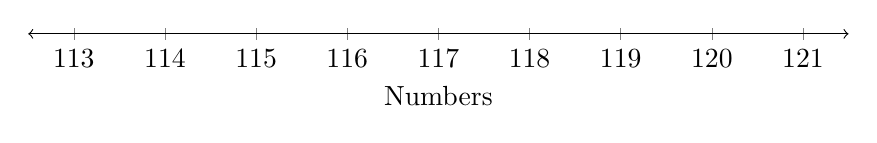
\begin{tikzpicture}
\begin{axis}[
axis y line=none,
axis lines=left,
axis line style={<->},
xmin=112.5,
xmax=121.5,
width=12cm,
height=4cm,
ymin=0,
ymax=1,
xlabel= Numbers,
scatter/classes={o={mark=*}},
restrict y to domain=0:1,
xtick={113,114,...,121}
]
\end{axis}
\end{tikzpicture}

\subsection{Examples of real Numbers}
$$\sqrt {81} = 9 $$
$$\sqrt {49} = 7 $$
$$\sqrt {25} = 5 $$
$$\sqrt {NegativeNumber} = NOT REAL$$ \footnote{Imaginary Numbers are for another lesson.}

\section{Word Problems}
\subsection{Adding}
These are words that you will want to recognize as additoin when reading a Math problem.
\begin{itemize}
\item Add
\item Sum
\item Total
\item Increase
\item Plus
\end{itemize}

\subsection{Subtracting}
Same as addition, these are words to recognoze when reading a word problen dealing with subtraction.
\begin{itemize}
	\item Subtract
	\item Minus
	\item Decrease
	\item Take Away
	\item Less than
	\item from
\end{itemize}

\subsection{Multiply}
Words that point to multiplication. 
\begin{itemize}
	\item Product
	\item Times 
	\item Of	
\end{itemize}
\subsection{Dividing}
Words to be recognized when one needs to divide. 
\begin{itemize}
	\item Divisible
	\item Divide
	\item Division
	\item Quotient
	\item Into
	\item Per
\end{itemize}

\section{Examples}
\subsection{simplify}
$$6 \times (7 - 4) \div 3 + 8 - 3 $$
$$6 \times (3) \div 3 + 8 - 3 $$
$$18  \div 3 + 8 - 3 $$
$$6 \div 3 + 8 - 3 $$
$$6 \div 8 - 3 $$
$$14 - 3$$
$$ 11$$

\subsection{Round the Numeral}
\begin{itemize}
	\item 85,379
\begin{itemize}
	\item Nearest Thousands Place:
	$85,000$
	\item Nearest Tens Place:
	$85,380$
	
\end{itemize}
\end{itemize}

\subsection{Expanded Notation}
\begin{itemize}
	\item This is the Standard Form: 85,379.
	\item This is the Expanded Notation: 
	
	$$80,000$$
	$$5,000$$
	$$300$$
	$$70$$
	$$9$$
\end{itemize}

\subsection{Fractions}
These are part of a whole.
\begin{equation}
	\frac {3}{5} 
\end{equation}

\subsection{Reducing Fractions}
Common Multiple.
\begin{equation}
	\frac {2 \div 2}{4 \div 2} = \frac{1}{2}
\end{equation}
	\begin{itemize}
		\item 2 = (2,4,6,8,10,12,...)
		\item 4 = (4,8,12,16,20,24,...)
	\end{itemize}
Common Factor.
	\begin{itemize}
		\item 2 = 1,2
		\item 4 = 1,2,4
	\end{itemize}
		2 is the Greatest Common Factor.
\begin{equation}
\frac {8}{24} = \frac {8 \div 8}{24 \div 8} = \frac {1}{3}
\end{equation}

\subsection{Simple Fractions}
\begin{itemize}
	\item Proper: Numerator is smaller than denominator. 
	\begin{itemize}
		\item \begin{equation}
			\frac{3}{4} 
		\end{equation}
		\item \begin{equation}
			\frac{1}{2}
		\end{equation}
	\end{itemize}
	\item Improper: Numerator ia larger than denominator. 
		\begin{itemize}
			\item \begin{equation}
			\frac{4}{3} 
			\end{equation}
			\item \begin{equation}
			\frac{2}{1}
			\end{equation}
		\end{itemize}
\end{itemize}

\subsection{Complex Fractions}
\begin{itemize}
	\item Mixed Numbers:
	\begin{equation}
	3 \frac{2}{5}
	\end{equation}
	\item Decimals:  3.5, 5.975
\end{itemize}

\subsection{Dividing  Fractions}
\begin{itemize}
	\item Reciprocal "multiplicative inverse"
	\begin{equation}
		\frac{A}{B} \div \frac{N}{D}  =  \frac{A}{B} \times \frac{D}{B}		
	\end{equation}
\end{itemize}

\subsection{Simplify:}
\begin{equation}
	\frac {10+7}{0} = \frac{17}{0}
\end{equation}
\begin{itemize}
	\item Anything Divided by Zero will always be Zero.
\end{itemize}

\subsection{Adding Fractions}
\begin{itemize}
	\item \begin{equation}
	\frac {2}{5} + \frac{3}{5} = 1
	\end{equation}
	\item \begin{equation}
		\frac{5}{8} + \frac{1}{8} = \frac{6}{8} = \frac{1}{4}
	\end{equation}
	
\end{itemize}




\end{document}
